\documentclass[10pt]{beamer}

\usetheme{default} % theme général du diaporama

% paquets pour le français
\usepackage[T1]{fontenc}
\usepackage[utf8]{inputenc}

\begin{document}

\begin{frame}
  \begin{figure}
    \centering
    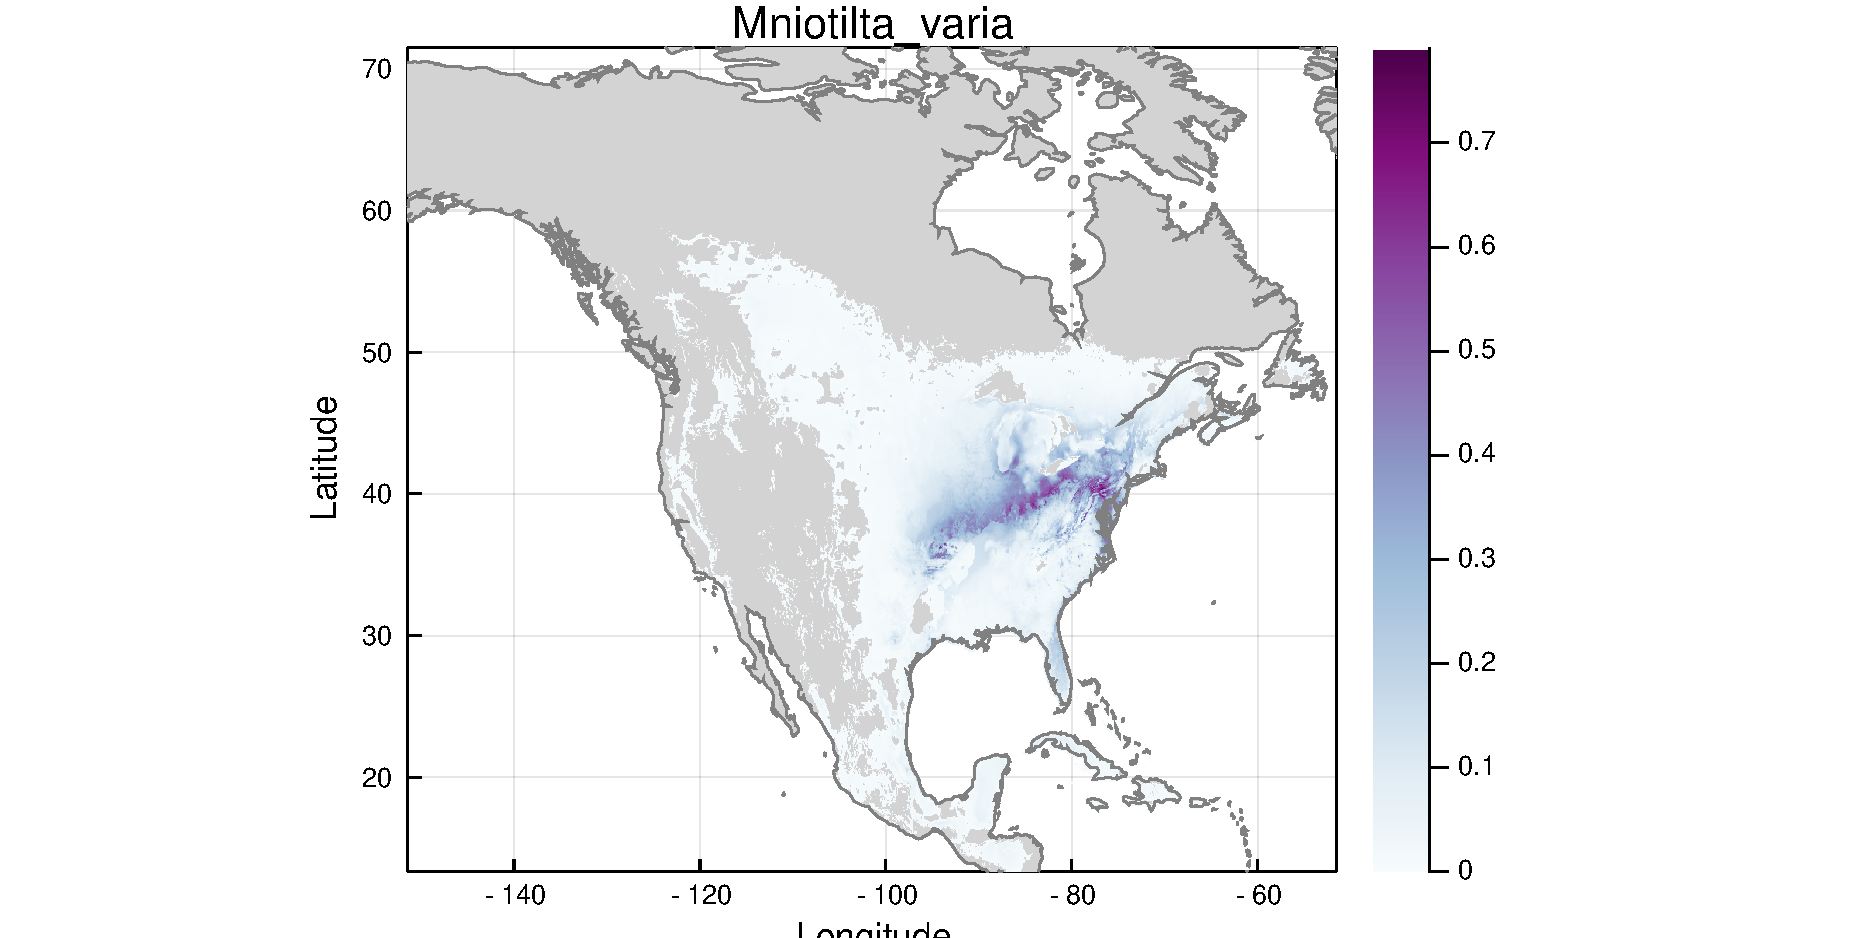
\includegraphics[scale=0.4]{fig/sdm-am-Mniotilta_varia.pdf}
  \end{figure}
\end{frame}

\begin{frame}
  \begin{figure}
    \centering
    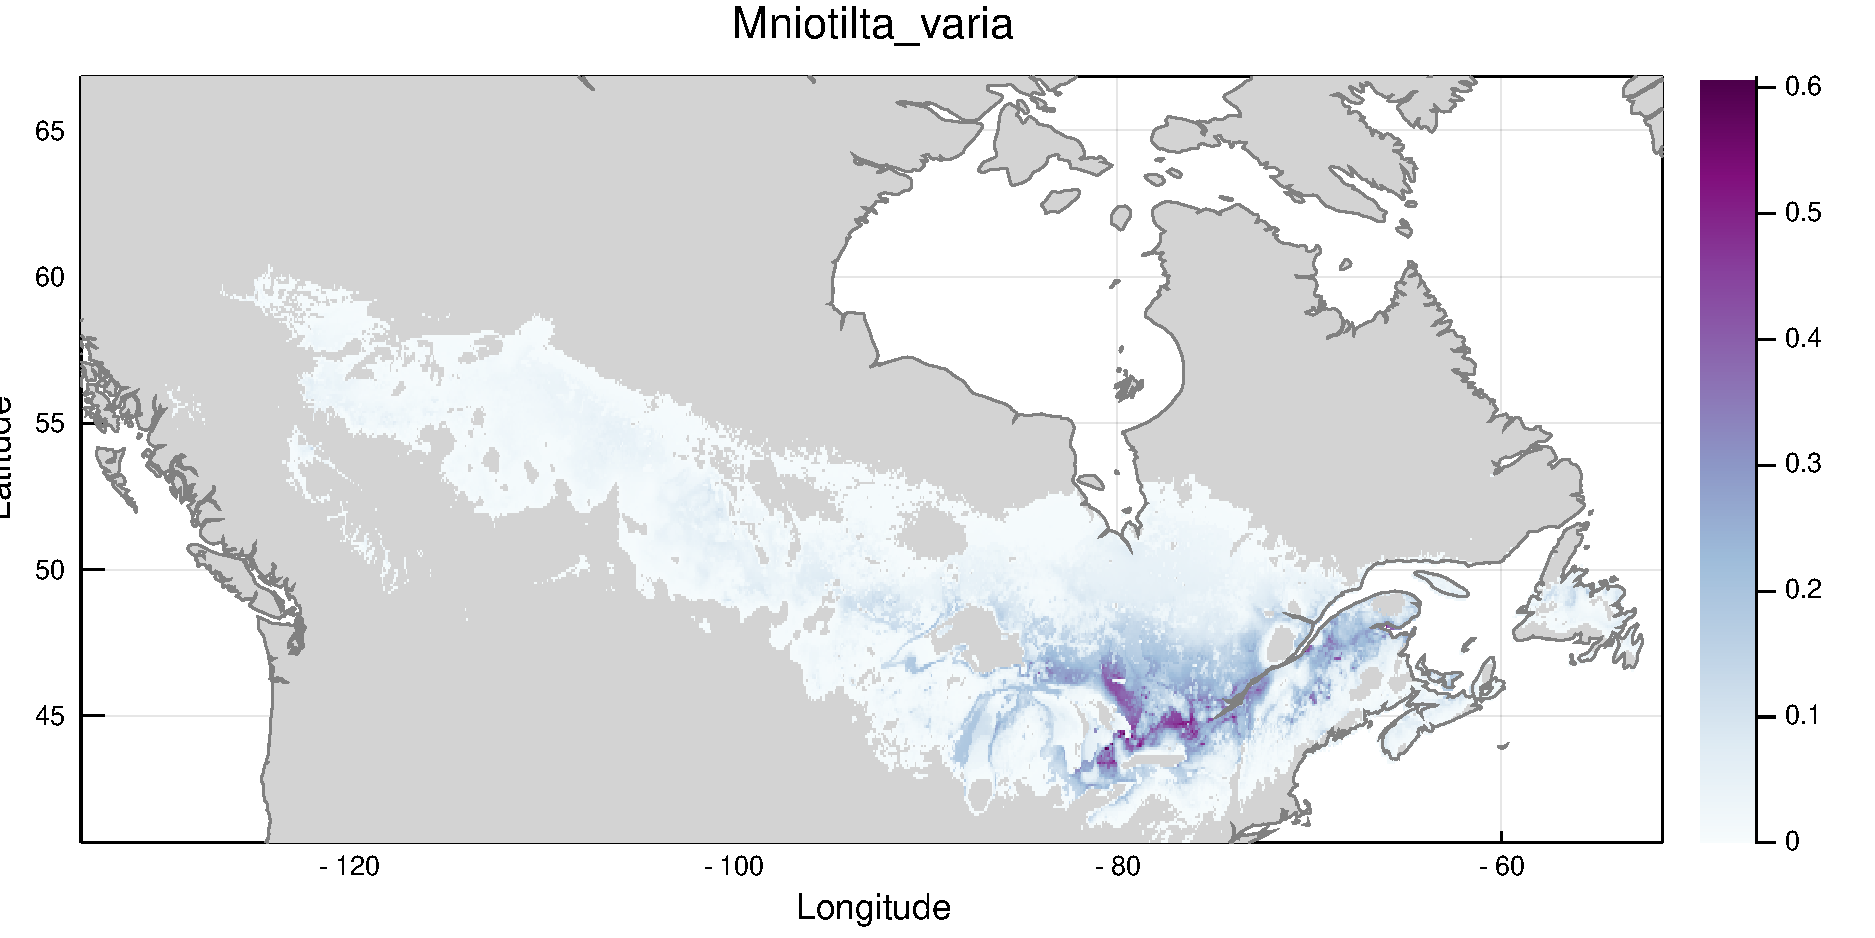
\includegraphics[scale=0.32]{fig/sdm-can-Mniotilta_varia.pdf}
  \end{figure}
\end{frame}

\begin{frame}
  \begin{figure}
    \centering
    \includegraphics[scale=0.32]{fig/comparison-am-larger2.pdf}
  \end{figure}
\end{frame}

\begin{frame}
  \begin{figure}
    \centering
    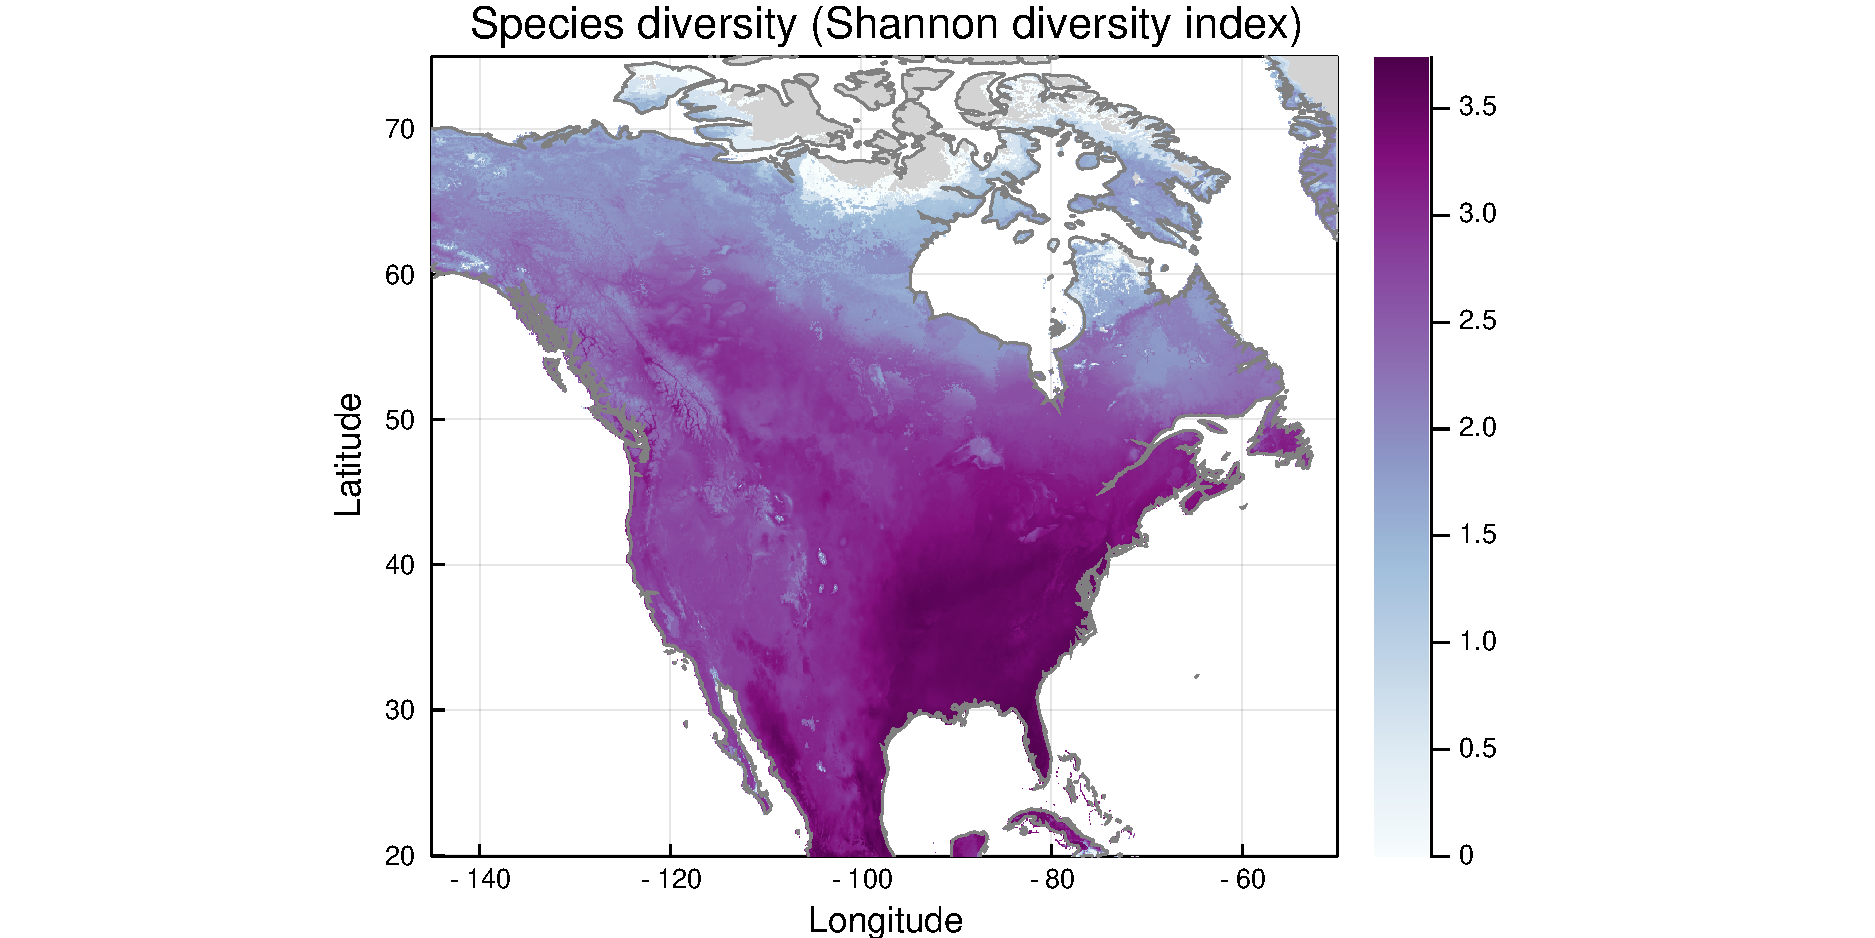
\includegraphics[scale=0.4]{fig/diversity-am-larger2.pdf}
  \end{figure}
\end{frame}

\begin{frame}
  \begin{figure}
    \centering
    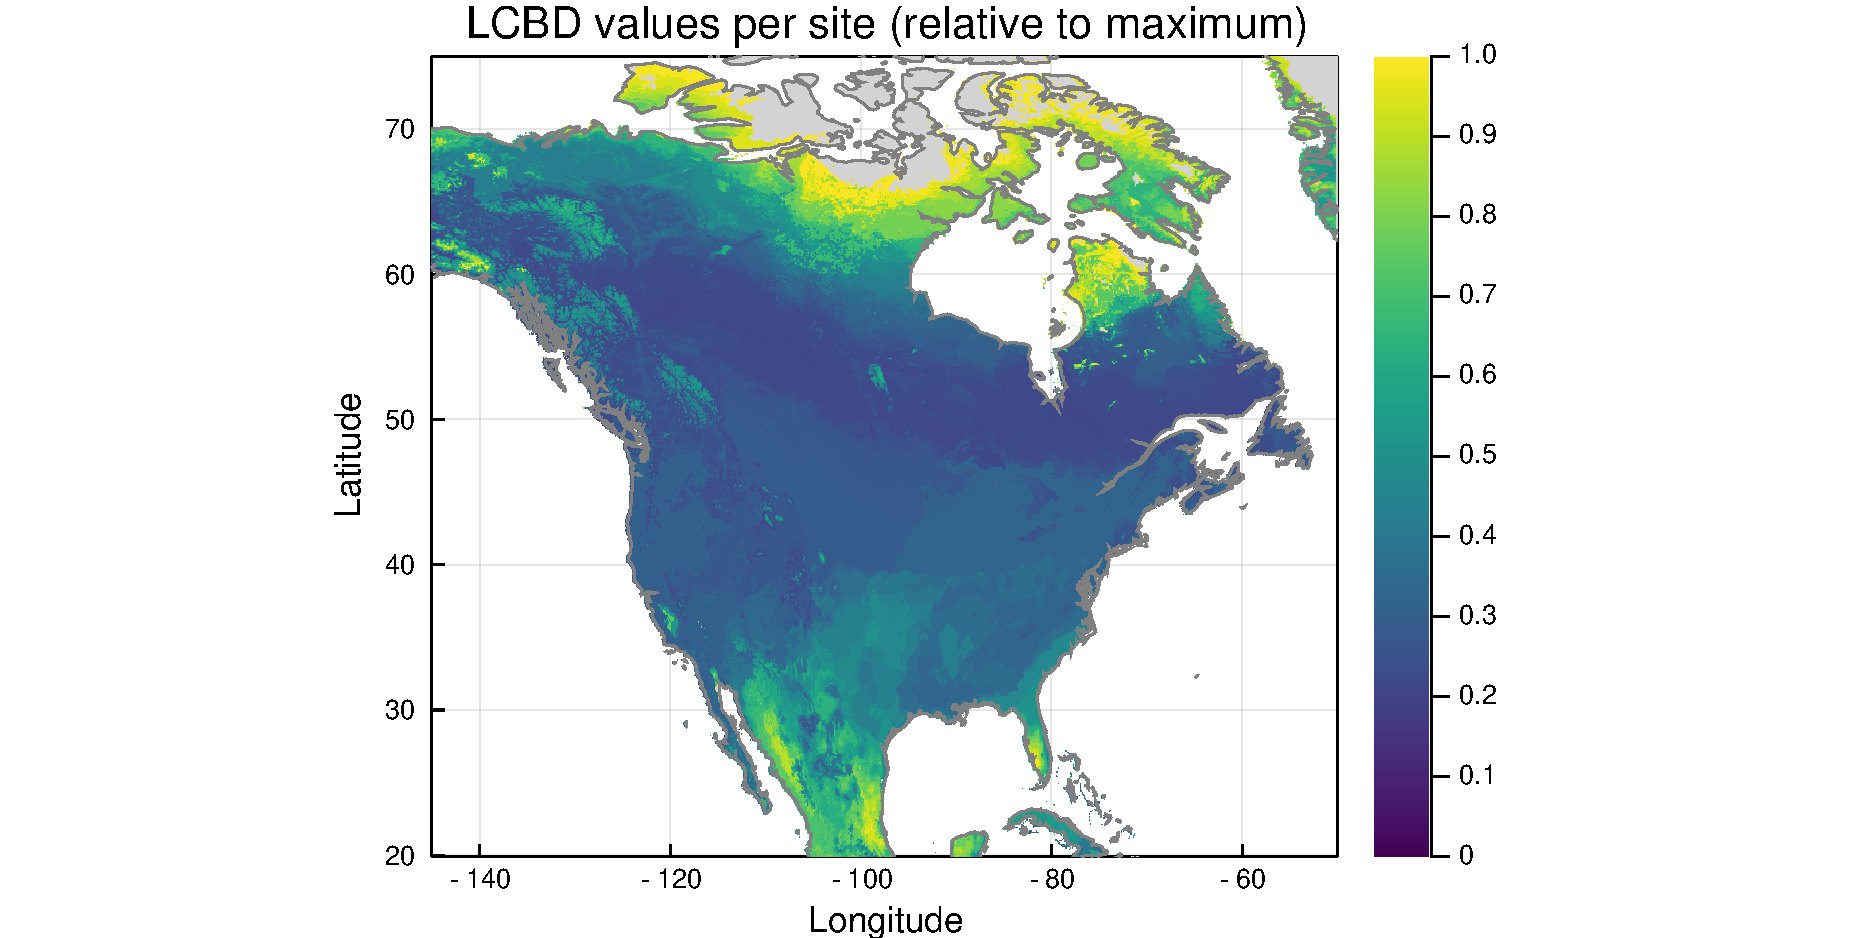
\includegraphics[scale=0.4]{fig/lcbd-am-larger2.pdf}
  \end{figure}
\end{frame}

\begin{frame}
  \begin{figure}
    \centering
    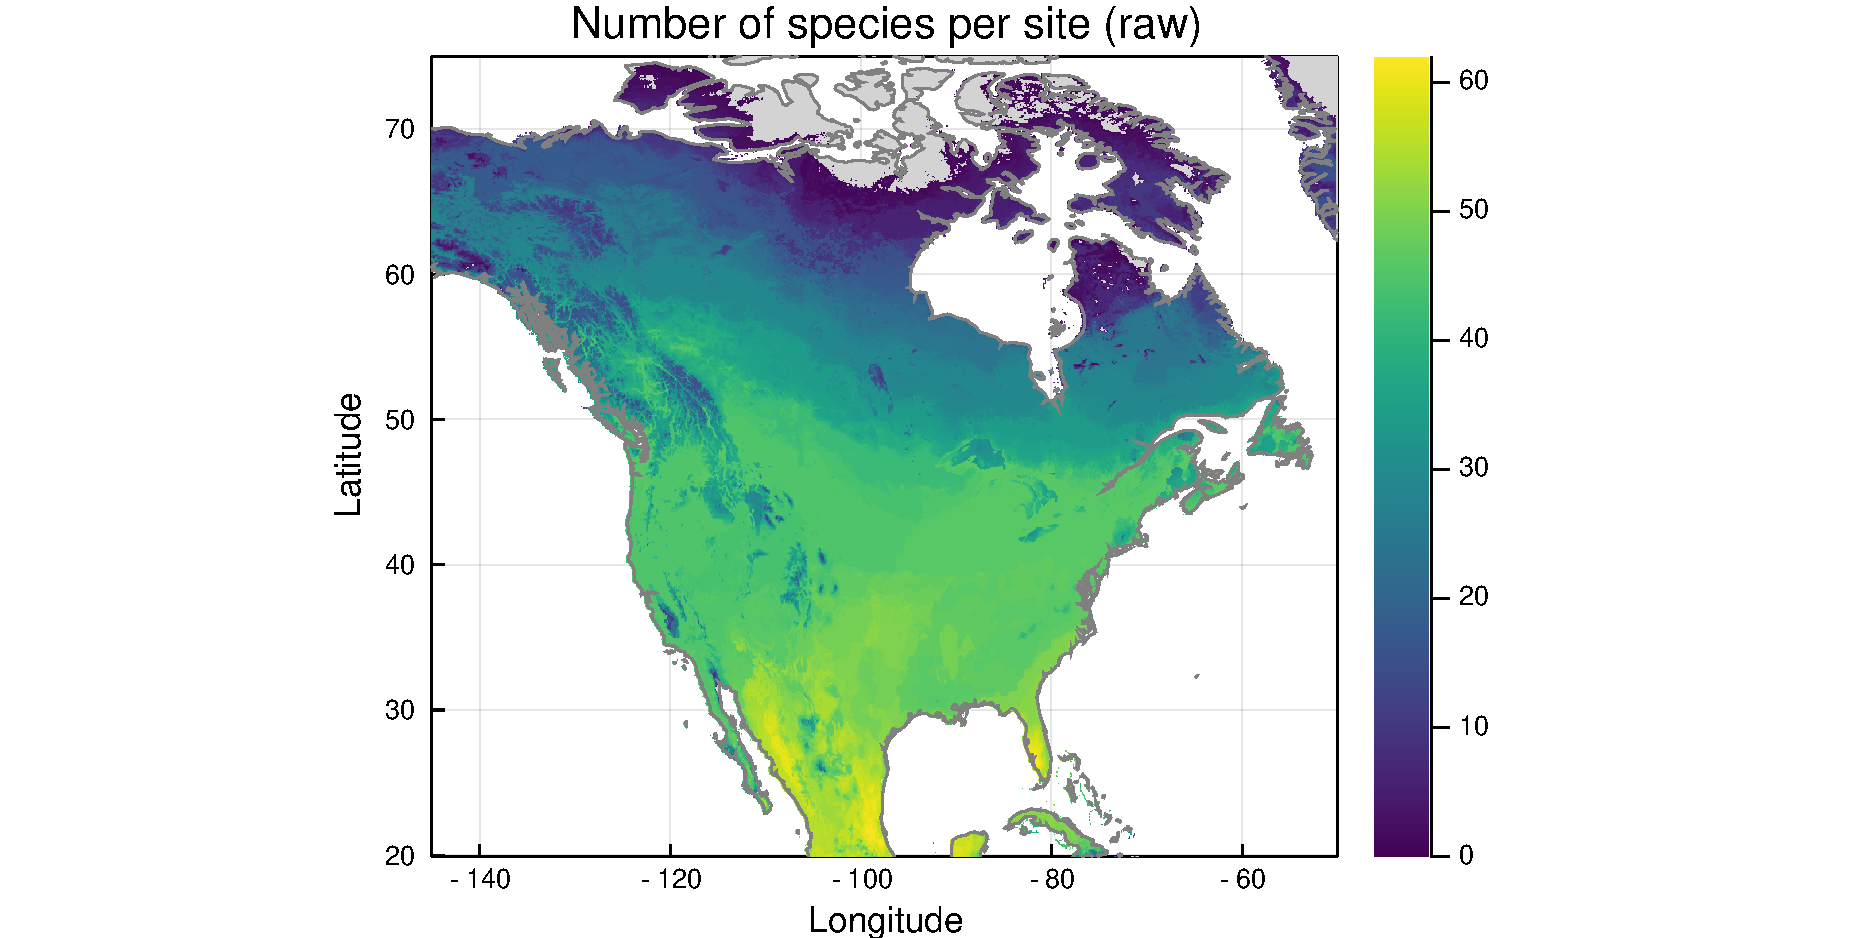
\includegraphics[scale=0.4]{fig/richness-am-larger2.pdf}
  \end{figure}
\end{frame}

\begin{frame}
  \begin{figure}
    \centering
    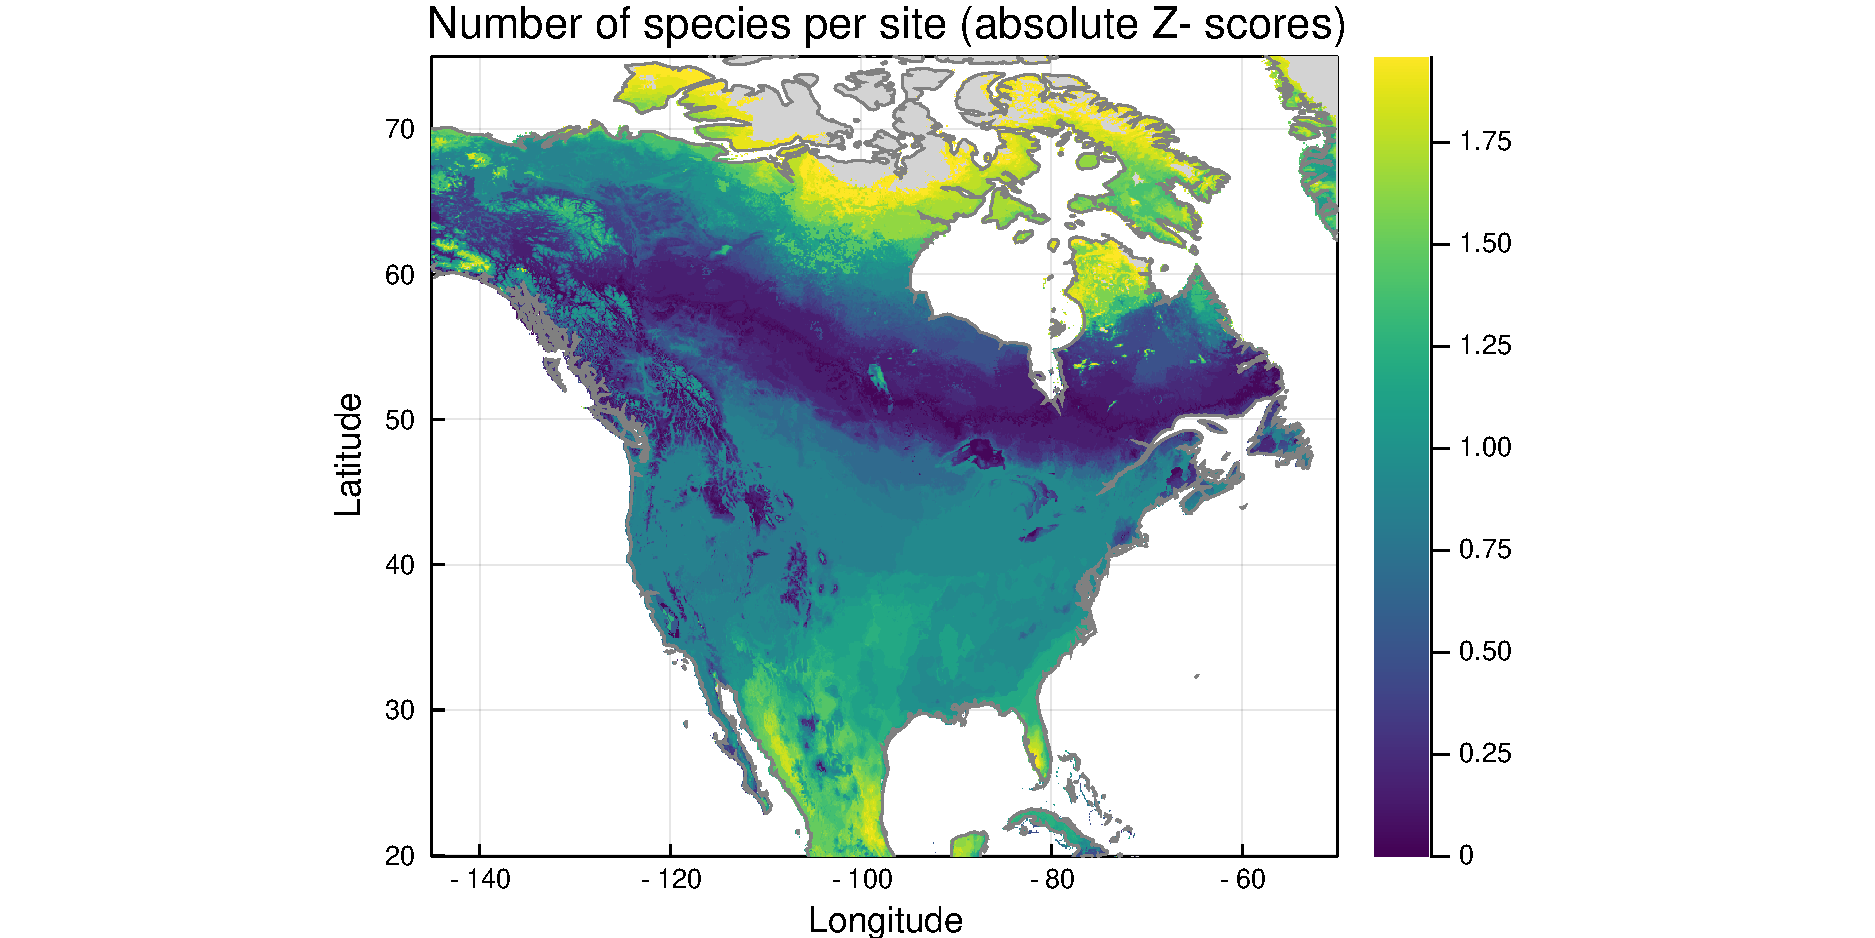
\includegraphics[scale=0.4]{fig/richness-am-larger2-zscores.pdf}
  \end{figure}
\end{frame}

\begin{frame}
  \begin{figure}
    \centering
    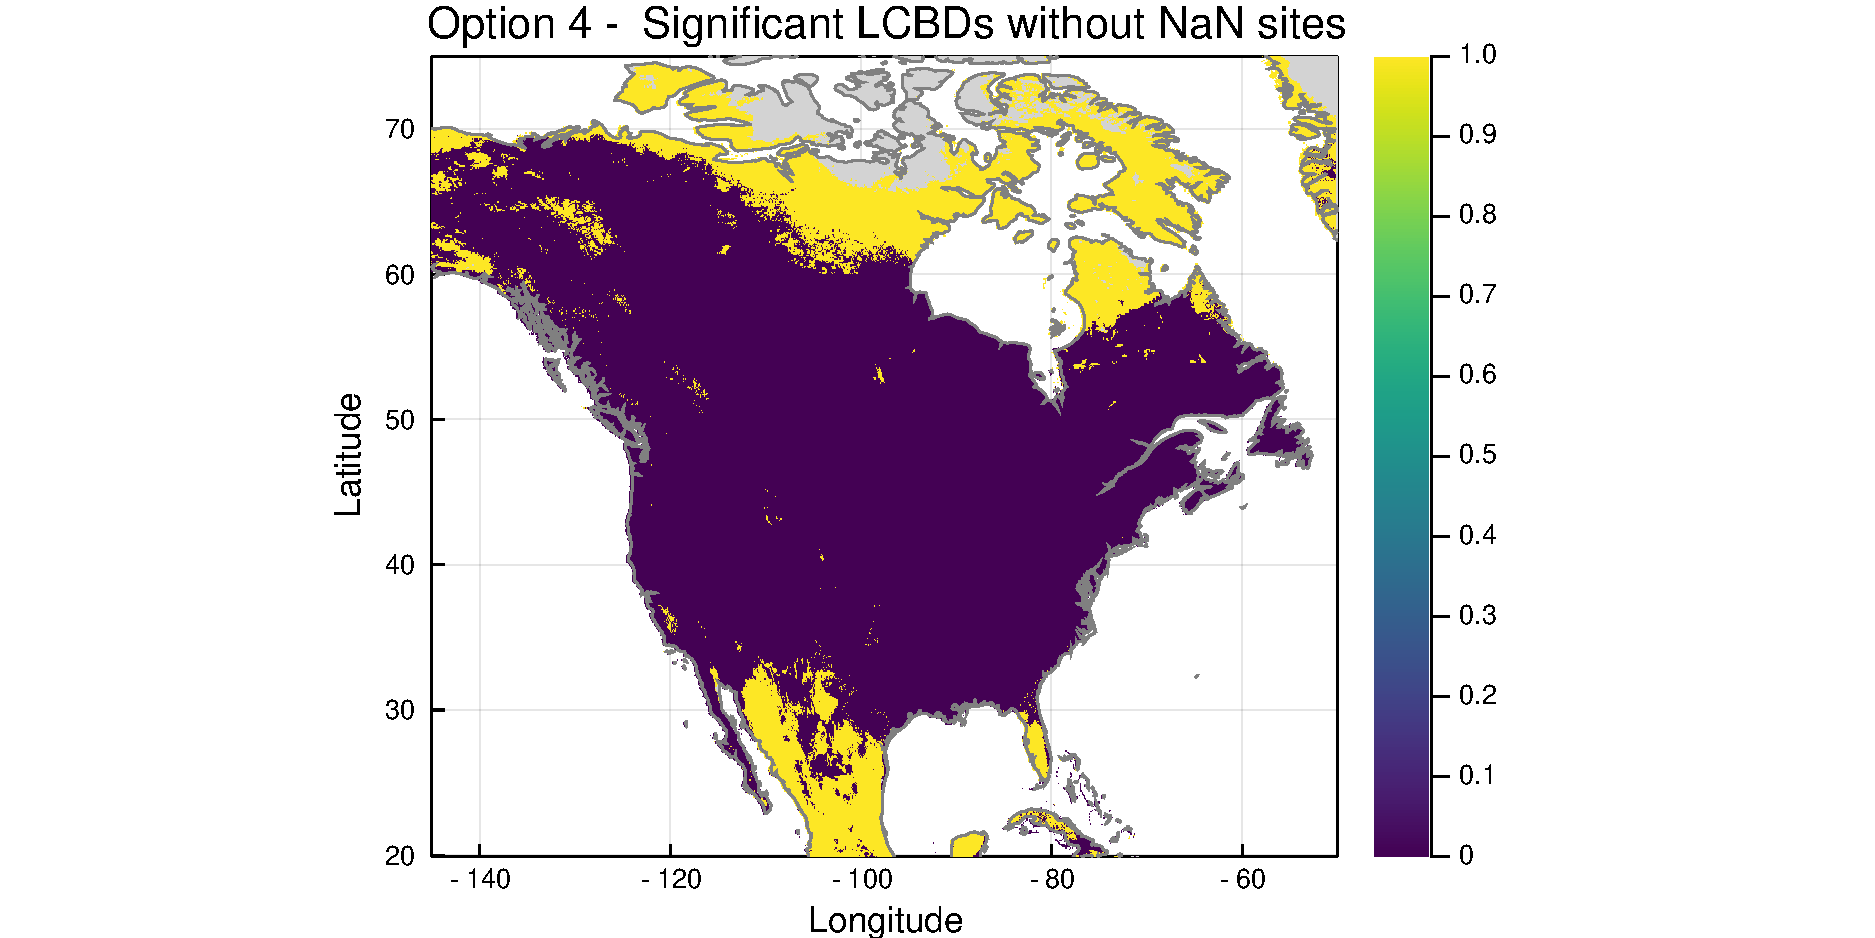
\includegraphics[scale=0.4]{fig/lcbd-am-larger2-significant.pdf}
  \end{figure}
\end{frame}

\end{document}
